\documentclass{article}
\usepackage{fancyhdr}
\usepackage{ctex}
\usepackage{listings}
\usepackage{graphicx}
\usepackage[a4paper, body={18cm,22cm}]{geometry}
\usepackage{amsmath,amssymb,amstext,wasysym,enumerate,graphicx}
\usepackage{float,abstract,booktabs,indentfirst,amsmath}
\usepackage{array}
\usepackage{booktabs}
\usepackage{multirow}
\usepackage{url}
\usepackage{diagbox}
\renewcommand\arraystretch{1.4}
\usepackage{indentfirst}
\setlength{\parindent}{2em}
\usepackage{enumerate}
\setmonofont{Consolas}
\usepackage{listings}
\usepackage{xcolor}
\usepackage{makecell}
\usepackage{enumitem}
\usepackage{tikz}
\usepackage{wrapfig}
\usepackage{tkz-euclide}
\usepackage{pgfplots}

\setfontfamily{\timesfont}{Times New Roman}

\begin{document}

\begin{center}
    \LARGE \textbf{\heiti 《数学建模及其{\timesfont MATLAB}实现》第一次课程作业} \\[0.5em]
    \large 李鹏达 10225101460
\end{center}

~\\

\paragraph{1.} 课堂上讨论了椅子腿连线呈正方形的情况,试讨论椅子腿连线呈矩形的情况.\\

\begin{wrapfigure}{r}{0.3\textwidth}
    \centering
    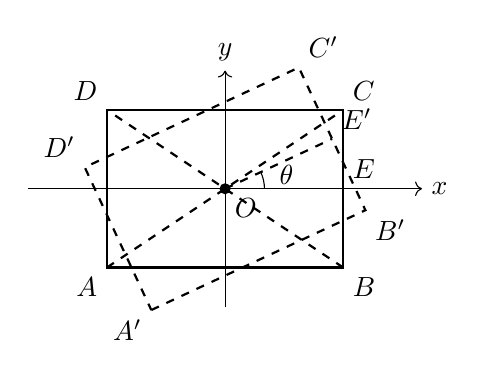
\begin{tikzpicture}
        % 定义矩形的顶点
        \coordinate (A) at (-1.5, -1);  % A的坐标:(-2, -1)
        \coordinate (B) at (1.5, -1);   % B的坐标:(2, -1)
        \coordinate (C) at (1.5, 1);    % C的坐标:(2, 1)
        \coordinate (D) at (-1.5, 1);   % D的坐标:(-2, 1)
        \coordinate (E) at (1.5, 0);  % O 的位置为 (0, 0)
        
        % 画矩形
        \draw[thick] (A) -- (B) -- (C) -- (D) -- cycle;
        
        % 画对角线
        \draw[thick, dashed] (A) -- (C);
        \draw[thick, dashed] (B) -- (D);
        
        % 计算交点 O
        \coordinate (O) at (0, 0);  % O 的位置为 (0, 0)
        \fill (O) circle (2pt) node[below right] {$O$}; % 标记 O
        
        % 标记顶点
        \node at (A) [below left] {$A$};
        \node at (B) [below right] {$B$};
        \node at (C) [above right] {$C$};
        \node at (D) [above left] {$D$};
        \node at (E) [above right] {$E$};
        
        % 画坐标轴
        \draw[->] (-2.5, 0) -- (2.5, 0) node[right] {$x$};  % x 轴
        \draw[->] (0, -1.5) -- (0, 1.5) node[above] {$y$};  % y 轴

        \begin{scope}[rotate around={25:(0,0)}]
            \coordinate (A') at (-1.5, -1);  % A的坐标:(-2, -1)
            \coordinate (B') at (1.5, -1);   % B的坐标:(2, -1)
            \coordinate (C') at (1.5, 1);    % C的坐标:(2, 1)
            \coordinate (D') at (-1.5, 1);   % D的坐标:(-2, 1)
            \coordinate (E') at (1.5, 0);  % O 的位置为 (0, 0)
            
            % 画矩形
            \draw[thick, dashed] (A') -- (B') -- (C') -- (D') -- cycle;
            \draw[thick, dashed] (O) -- (E');

            \node at (A') [below left] {$A'$};
            \node at (B') [below right] {$B'$};
            \node at (C') [above right] {$C'$};
            \node at (D') [above left] {$D'$};
            \node at (E') [above right] {$E'$};
        \end{scope}

        \tkzMarkAngle[size=0.5](E,O,E')  % 标记 ∠BOC
        \tkzLabelAngle[pos=0.8](E,O,E'){$\theta$}  % 显示角度符号
    \end{tikzpicture}

    \caption{\kaishu 椅子腿的连线呈矩形}
    \label{fig:chair}
\end{wrapfigure}

\noindent{\heiti 解答:}

如图\ref{fig:chair} 所示,设椅子腿连线呈矩形$ABCD$.设对角线$AC$与$BD$的交点为$O$, $BC$的中点为$E$. 以$O$为原点,$OE$的方向为$x$轴,建立平面直角坐标系.设 $OE$与$x$轴的夹角为$\theta$,则可以用$\theta$来表示椅子的位置.例如,椅子绕$O$旋转角度$\theta$后,矩形$ABCD$转至$A'B'C'D'$的位置.

根据矩形的对称性,设$A$, $B$两脚离地面的距离之和为$f(\theta)$, $C$, $D$两脚离地面的距离之和为$g(\theta)$.由假设 2, $f$ 和 $g$ 都是连续函数.由假设 3, 椅子在任何位置至少有三只脚着地,所以对于任意的 $\theta$, $f(\theta)$ 和 $g(\theta)$ 中至少有一个为零.当$\theta = 0 $ 时,不妨设 $g(0) = 0$, $f(0) > 0$,而当椅子旋转 $180^\circ$ 后, $AB$ 与 $CD$ 互换,于是 $f(\pi) = 0$, $g(\pi) > 0$.

设 $h(\theta) = f(\theta) - g(\theta)$, 则 $h(0) > 0$, $h(\pi) < 0$.由连续函数的性质,存在 $\theta_0 \in (0, \pi)$, 使得 $h(\theta_0) = 0$.即存在 $\theta_0 \in (0, \pi)$, 使得 $f(\theta_0) = g(\theta_0)$, 即椅子在 $\theta_0$ 位置时, 两脚离地面的距离相等.\\\\

\paragraph{2.} 在实物交换模型中,无差别曲线族表现为下凸.请分析,无差别曲线族表现为上凸代表什么?\\

\noindent{\heiti 解答:}

\begin{wrapfigure}{r}{0.3\textwidth}
    \centering
    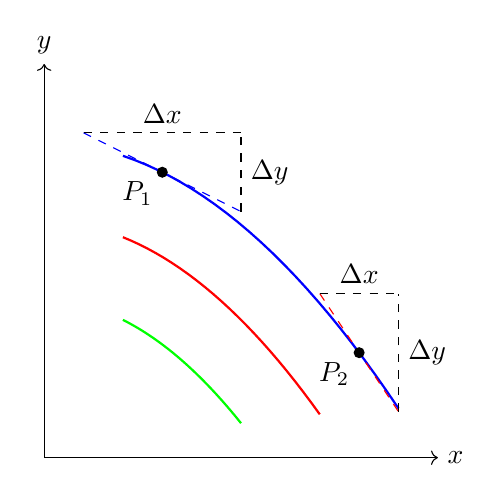
\begin{tikzpicture}
        % 绘制无差别曲线
        \draw[blue, thick, domain=1:4.5] plot (\x, {4 - \x^2/6}) node[right] {};
        \draw[red, thick, domain=1:3.5] plot (\x, {3 - \x^2/5}) node[right] {};
        \draw[green, thick, domain=1:2.5] plot (\x, {2 - \x^2/4}) node[right] {};
        
        % 选择的两点
        \coordinate (P1) at (1.5, {4 - 1.5^2/6});
        \coordinate (P2) at (4, {4 - 4^2/6});
        
        % 绘制切线
        % 切线 A 的斜率
        \pgfmathsetmacro{\slopeA}{-(1.5/3)};
        % 切线 B 的斜率
        \pgfmathsetmacro{\slopeB}{-(4.5/3)};
        
        % 切线方程
        \draw[blue, dashed] plot[domain=0.5:2.5] (\x, {\slopeA*(\x - 1.5) + (4 - 1.5^2/6)}) node[right] {};
        \draw[red, dashed] plot[domain=3.5:4.5] (\x, {\slopeB*(\x - 4) + (4 - 4^2/6)}) node[right] {};

        \coordinate (C) at (0.5, {\slopeA*(0.5 - 1.5) + (4 - 1.5^2/6)});
        \coordinate (D) at (2.5, {\slopeA*(2.5 - 1.5) + (4 - 1.5^2/6)});
        \coordinate (E) at (2.5, {\slopeA*(0.5 - 1.5) + (4 - 1.5^2/6)});
        \coordinate (F) at (3.5, {\slopeB*(3.5 - 4) + (4 - 4^2/6)});
        \coordinate (G) at (4.5, {\slopeB*(4.5 - 4) + (4 - 4^2/6)});
        \coordinate (H) at (4.5, {\slopeB*(3.5 - 4) + (4 - 4^2/6)});

        \draw[black, dashed] (D) -- (E) node[midway, right] {$\Delta y$};
        \draw[black, dashed] (C) -- (E) node[midway, above] {$\Delta x$};

        \draw[black, dashed] (F) -- (H) node[midway, above] {$\Delta x$};
        \draw[black, dashed] (G) -- (H) node[midway, right] {$\Delta y$};
        
        % 在切点上标记
        \fill[black] (P1) circle (2pt) node[below left] {$P_1$};
        \fill[black] (P2) circle (2pt) node[below left] {$P_2$};
        
        % 设置坐标轴
        \draw[->] (0, 0) -- (5, 0) node[right] {$x$};
        \draw[->] (0, 0) -- (0, 5) node[above] {$y$};
        
    \end{tikzpicture}
    \caption{\kaishu 上凸无差别曲线族}
    \label{fig:concave}
\end{wrapfigure}

如图 \ref{fig:concave} 所示,设无差别曲线族表现为上凸.取同一条曲线上的两点$P_1$和$P_2$$(P_{1x}<P_{2x})$,做如图所示的切线三角形.

在$P_1$处,其占有的$x$较少, $y$较多, $\Delta x > \Delta y$, 说明他倾向于用较多的$x$换较少的$y$;而在$P_2$处,其占有的$x$较多, $y$较少, $\Delta x < \Delta y$,说明他倾向于用较少的$x$换较多的$y$.

在这种情况下,他占有的$x$越少,反而愿意用更多的$x$换取更少的$y$,这种``物以稀为贱,物以多为贵''的情况,在实际中是不合理的.

因此,无差别曲线族表现为上凸,代表了一种不合理的情况.


\end{document}